\section{问题一：单点往返运输能力与时间优先货箱组批优化}
\label{sec:q1}

\subsection{问题分析与求解思路}

本问的核心是将连续的运输能力边界转化为离散的货箱组批方案，并在完整交付的前提下说明架次数、能耗和累计作业时间之间的取舍。每个架次只能沿 $O01\to S_i\to O01$ 直接往返，去程携带该批货箱、交付后空载返回；不同服务区之间不能合批。本问不引入实体无人机数量、共享电池周转或多机并行调度，因而累计作业时间是各架次作业时间之和，不是所有任务的最晚完成时刻。逐箱时限亦不作为本问的优化约束。

依据题面附录 2 的统一计算规则，首先由节点与原始 DEM 确定水平距离和巡航海拔，计算不同机型的时间与能耗；再利用能耗随载荷的单调性求最大安全载荷。随后，以同类货箱的数量向量枚举可行装载模式，通过多目标动态规划获得各区完整的非支配目标集合，最后合成全局 Pareto 前沿。此处采用精确枚举而非随机启发式搜索，是因为本问不存在跨区耦合，且每区物资类别少、需求状态规模有限，可以在保留所有有效权衡的同时给出可回溯方案。

决策阶段采用\textbf{累计作业时间优先、架次数次之、能耗再次之}的字典序规则。该规则表达尽量减少累计飞行及装卸交接投入的偏好，并不是题面强制规定的唯一价值排序。因此，保留架次优先、能耗优先与归一化等权规则作为对照，先展示完整前沿，再说明推荐理由和偏好改变时的方案切换，避免先设权重后遗漏有效方案。

\subsection{地形约束下的往返时间与能耗}
\subsubsection{直线航段、巡航海拔与作业高度}

附件给出 1 个调度中心、15 个服务区与 80 个不可拆货箱，合计质量为 $758\,\mathrm{kg}$、体积为 $2.011\,\mathrm{m^3}$。节点经纬度按 WGS84 椭球的局部距离公式转换：在两点平均纬度 $\bar\varphi$ 处，取子午圈与卯酉圈曲率半径 $M(\bar\varphi)$、$\mathcal N(\bar\varphi)$，有
\begin{equation}
 d_i=\sqrt{[M(\bar\varphi)\Delta\varphi]^2+
 [\mathcal N(\bar\varphi)\cos\bar\varphi\,\Delta\lambda]^2}.
 \label{eq:q1-distance}
\end{equation}
角度差在式中取弧度。对节点间的水平直线遍历其实际经过的原始 DEM 像元集合 $\mathcal C_i$，按题意确定
\begin{equation}
 H_i=\max_{c\in\mathcal C_i}z_c+50,
 \qquad z_i^{\rm op}=z_i+30,\quad z_O^{\rm op}=z_O.
 \label{eq:q1-height}
\end{equation}
由此得到去程爬升高度 $h_i^O=H_i-z_O$ 和回程爬升高度 $h_i^S=H_i-z_i^{\rm op}$；去程下降高度为 $h_i^S$，回程下降高度为 $h_i^O$。本数据的四类高度差均非负。最高像元决定巡航海拔，服务区自身海拔不能替代沿线地形扫描。

图~\ref{fig:q1-terrain}以三维视图呈现地形与航线，图~\ref{fig:q1-profiles}给出三个具有不同几何特征的航段。S008 距离最远，而 S014 的巡航海拔最高，说明远距离与大爬升是不同的负担来源，不能只按距离排序判断运输能力。
\begin{figure}[!htbp]
 \centering
 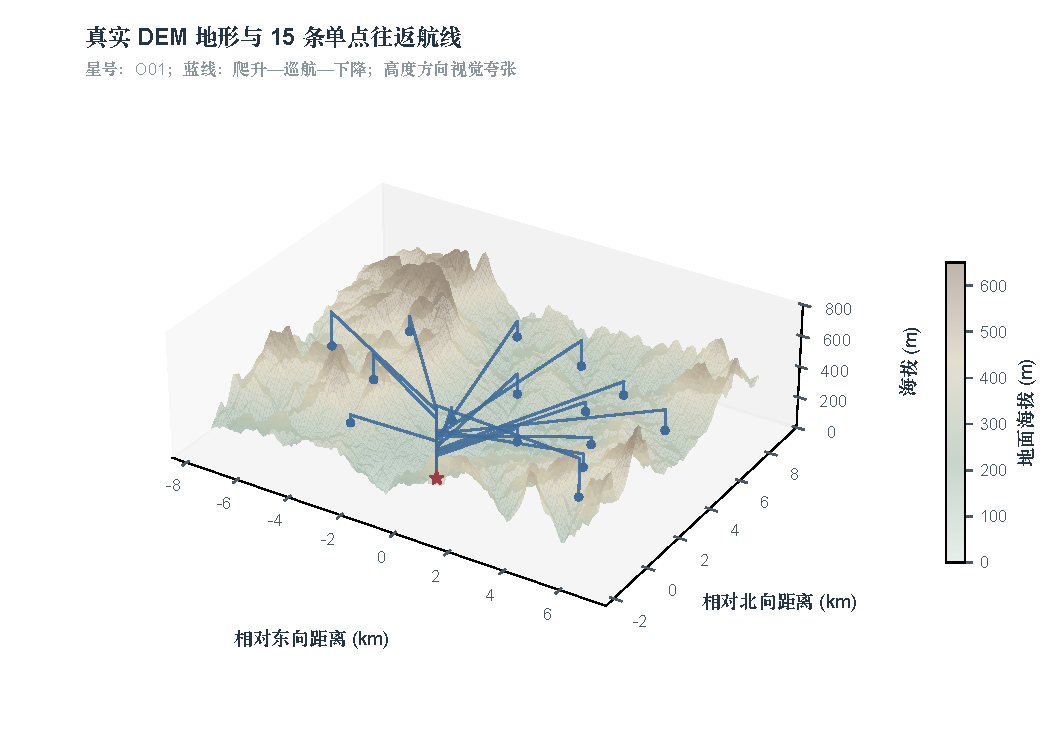
\includegraphics[width=\linewidth]{figures/q1_terrain3d.pdf}
 \caption{真实 DEM 地形与 15 条单点往返计划航线。坐标以 O01 为原点；高度方向作视觉夸张，轴值仍为实际海拔。地形显示采用 $4\times4$ 像元块最大值聚合，航线叠加前置以便辨认；运输计算始终采用原始分辨率。}
 \label{fig:q1-terrain}
\end{figure}
\begin{figure}[!htbp]
 \centering
 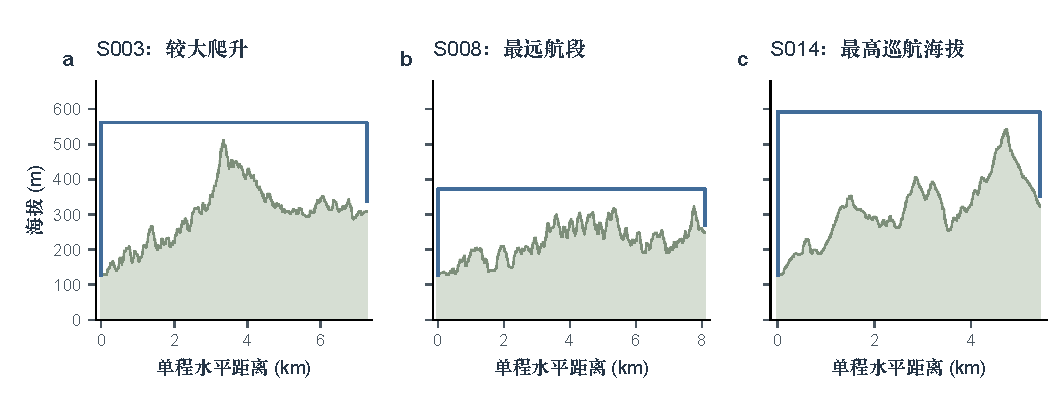
\includegraphics[width=\linewidth]{figures/q1_profiles.pdf}
 \caption{代表航段的地形剖面与去程三阶段包线。S003 展示较大爬升，S008 为最远航段，S014 为最高巡航海拔航段。剖面曲线为沿线 400 点显示采样，巡航海拔依据全部经过像元的最大值确定。}
 \label{fig:q1-profiles}
\end{figure}

\subsubsection{载荷相关能耗与累计作业时间}

记机型 $g$ 的结构最大载荷为 $Q_g$，空载与满载标准航程为 $L_g^0,L_g^F$，单组电池可用能量为 $E_g^{\rm use}$。直接采用题面给定的等效航程关系
\begin{equation}
 L_g(q)=L_g^0-(L_g^0-L_g^F)(q/Q_g)^{3/2},\qquad 0\le q\le Q_g.
 \label{eq:q1-range}
\end{equation}
水平能耗按距离占等效航程的比例折算，爬升附加能耗按有效质量克服重力做功并除以爬升效率计算。将去程载荷 $q$ 与回程空载分别代入，往返能耗为
\begin{equation}
 E_{gi}(q)=d_iE_g^{\rm use}\left[\frac{1}{L_g(q)}+\frac{1}{L_g^0}\right]
 +\frac{g_0[(m_g^0+q)h_i^O+m_g^0h_i^S]}{3.6\times10^6\eta_g^{\uparrow}}.
 \label{eq:q1-energy}
\end{equation}
其中 $m_g^0$ 为含电池空载总质量，$g_0=9.81\,\mathrm{m/s^2}$，分母换算为 kWh。下降能耗效率为零表示不另计下降附加能耗，不能据此忽略下降时间。返航安全要求为 $E_{gi}(q)\le(1-\rho_g)E_g^{\rm use}$，基准 $\rho_g=0.20$。

根据三阶段串行飞行规则，装载 $n$ 箱的架次累计作业时间为
\begin{align}
 t_{gi}^{\rm fly}&=\frac{h_i^O+h_i^S}{v_g^{\uparrow}}+
 \frac{2d_i}{v_g^c}+\frac{h_i^O+h_i^S}{v_g^{\downarrow}},\label{eq:q1-flighttime}\\
 T_{gi}(n)&=t_g^{\rm prep}+t_g^{\rm hand}+t_{gi}^{\rm fly}
       +n(t_g^{\rm load}+t_g^{\rm box}).\label{eq:q1-time}
\end{align}
各机型参数均取运输无人机附件。该时间模型同时计入固定准备、逐箱装载和交接，因此减少架次会减少重复的固定作业，但不同机型速度及交接参数不同，最少架次不必然意味着最少累计时间。

\subsection{最大安全载荷及限制来源}

对固定机型与服务区，$L_g(q)$ 随 $q$ 递减且保持正值，式~\eqref{eq:q1-energy}中的水平能耗递增，爬升项也随 $q$ 递增。因此 $E_{gi}(q)$ 连续且严格递增，最大安全载荷可表示为
\begin{equation}
 q_{gi}^{\max}(\rho_g)=
 \begin{cases}
 \text{不可行},&E_{gi}(0)>(1-\rho_g)E_g^{\rm use},\\
 Q_g,&E_{gi}(Q_g)\le(1-\rho_g)E_g^{\rm use},\\
 E_{gi}^{-1}((1-\rho_g)E_g^{\rm use}),&\text{其余情形}.
 \end{cases}
 \label{eq:q1-qmax}
\end{equation}
在第三种情形下，于 $[0,Q_g]$ 内作 60 次二分求根，结果另以 Brent 求根交叉核验。最大载荷是连续质量上界；具体货箱组合还需同时满足体积与不可拆分约束，不能把该上界直接视作一定能装满的实际载荷。

表~\ref{tab:q1-payload}给出全部 45 个机型--服务区组合的结果，图~\ref{fig:q1-payload}显示其限制来源。A 型在全部服务区均受 $25\,\mathrm{kg}$ 结构上限约束；B 型仅在 S008 受能量约束，载荷降至 $28.80\,\mathrm{kg}$；C 型在 S002、S003、S004、S008 和 S012 受能量约束，其余服务区可达 $80\,\mathrm{kg}$。因此，大载荷机型有利于合批，但其优势也受距离和爬升能耗共同制约。
\begin{table}[!htbp]
\centering
\caption{基准返航安全余量下的最大安全载荷}
\label{tab:q1-payload}
\small
\setlength{\tabcolsep}{4pt}
\renewcommand{\arraystretch}{1.10}
\begin{tabular}{@{}lrrrrr@{}}
\toprule
服务区 & 距离（km） & 巡航海拔（m） & A（kg） & B（kg） & C（kg） \\
\midrule
S001 & 3.05 & 273.06 & 25.00 & 30.00 & 80.00 \\
S002 & 7.41 & 308.95 & 25.00 & 30.00 & 68.86 \\
S003 & 7.26 & 561.80 & 25.00 & 30.00 & 68.21 \\
S004 & 7.71 & 398.24 & 25.00 & 30.00 & 63.70 \\
S005 & 5.28 & 326.41 & 25.00 & 30.00 & 80.00 \\
S006 & 3.19 & 366.10 & 25.00 & 30.00 & 80.00 \\
S007 & 4.53 & 511.97 & 25.00 & 30.00 & 80.00 \\
S008 & 8.08 & 372.91 & 25.00 & 28.80 & 58.90 \\
S009 & 5.71 & 293.23 & 25.00 & 30.00 & 80.00 \\
S010 & 4.78 & 435.64 & 25.00 & 30.00 & 80.00 \\
S011 & 2.81 & 295.36 & 25.00 & 30.00 & 80.00 \\
S012 & 7.39 & 413.30 & 25.00 & 30.00 & 68.12 \\
S013 & 4.85 & 399.18 & 25.00 & 30.00 & 80.00 \\
S014 & 5.42 & 591.95 & 25.00 & 30.00 & 80.00 \\
S015 & 6.01 & 571.80 & 25.00 & 30.00 & 80.00 \\
\bottomrule
\end{tabular}
\par\smallskip{\footnotesize 最大载荷仅表示质量与能量允许的连续上界；实际组批还须满足体积约束。}
\end{table}

\begin{figure}[!htbp]
 \centering
 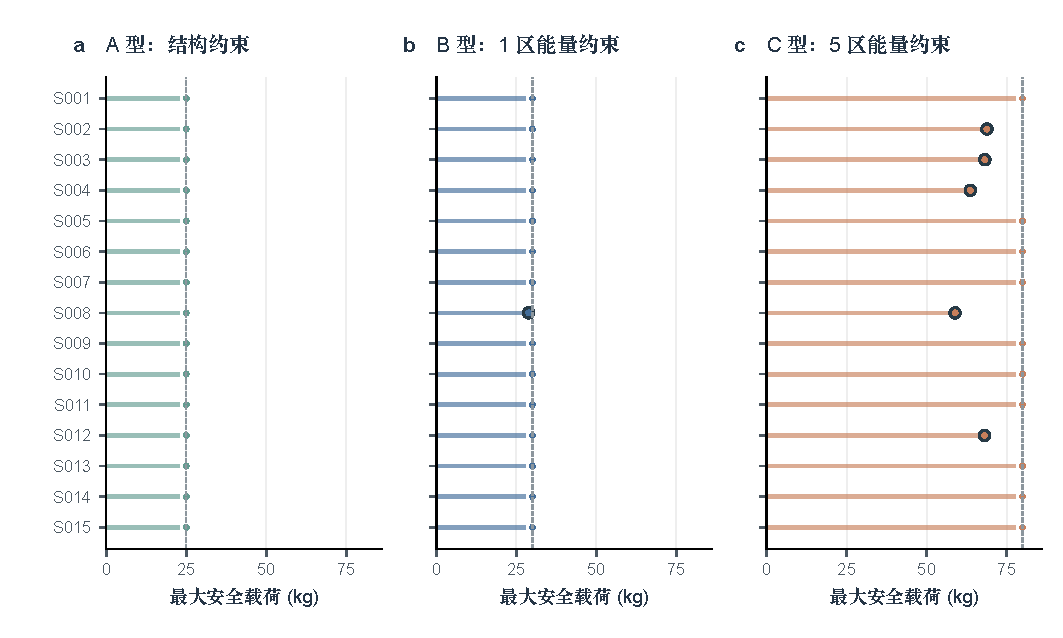
\includegraphics[width=\linewidth]{figures/q1_payload.pdf}
 \caption{三种机型在全部服务区的最大安全载荷。三面板共享质量尺度，虚线为结构载荷上限，深色边框点表示能量约束先于结构上限生效；基准返航安全余量为 20\%。}
 \label{fig:q1-payload}
\end{figure}

\subsection{不可拆货箱的多目标精确组批模型}
\subsubsection{装载模式与整数规划表述}

逐箱核验表明，同一服务区内同类物资的单箱质量、体积一致。本问又不约束逐箱送达时刻，因此可将箱号组合压缩为四类物资的计数向量，而不损失质量、体积或代价信息。记需求向量为 $\boldsymbol r_i$，单箱质量、体积分别为 $m_k,v_k$。一个装载模式为 $\pi=(g,\boldsymbol n_\pi)$，其中 $\boldsymbol n_\pi$ 是非零非负整数向量；模式集合 $\mathcal P_i$ 由下列条件限定：
\begin{equation}
 \boldsymbol n_\pi\le\boldsymbol r_i,\qquad
 q_\pi=\sum_km_kn_{\pi k}\le q_{gi}^{\max},\qquad
 \sum_kv_kn_{\pi k}\le V_g.
 \label{eq:q1-pattern}
\end{equation}
最大安全载荷已同时包含结构质量与返航能量限制，但在最终方案检查时仍直接复算能耗，不仅检查载荷上界。

令 $x_{i\pi}$ 为服务区 $i$ 使用模式 $\pi$ 的次数，则三目标整数规划为
\begin{align}
 \min\ (N,E,T)&=\left(\sum_{i,\pi}x_{i\pi},\;
 \sum_{i,\pi}E_{gi}(q_\pi)x_{i\pi},\;
 \sum_{i,\pi}T_{gi}\!\left(\sum_kn_{\pi k}\right)x_{i\pi}\right),\label{eq:q1-mip}\\
 \text{s.t.}\quad \sum_{\pi\in\mathcal P_i}n_{\pi k}x_{i\pi}&=r_{ik},\qquad
 x_{i\pi}\in\mathbb Z_{\ge0}.\label{eq:q1-cover}
\end{align}
等式约束要求每类需求恰好满足，模式仅属于一个服务区，从而排除跨区合批。回溯后，将相应类型的真实箱号一一填入模式，再核对 80 个箱号无遗漏、无重复。这一步把计数方案落实为逐箱方案，而不是仅给出各区总质量。

\subsubsection{剩余需求状态与 Pareto 递推}

设 $F_i(\boldsymbol r)$ 为剩余需求 $\boldsymbol r$ 的非支配代价集合，模式代价为 $\boldsymbol c_\pi=(1,E_\pi,T_\pi)$，则
\begin{equation}
 F_i(\boldsymbol r)=\operatorname{ND}\!\left\{
 \boldsymbol c_\pi+\boldsymbol f:
 \boldsymbol n_\pi\le\boldsymbol r,\quad
 \boldsymbol f\in F_i(\boldsymbol r-\boldsymbol n_\pi)
 \right\},\qquad F_i(\boldsymbol0)=\{(0,0,0)\}.
 \label{eq:q1-dp}
\end{equation}
$\operatorname{ND}$ 删除被其他向量逐分量不大于、且至少一个分量严格更小的解，并合并相同目标向量。对同一箱数向量，先删除能耗和时间均不占优的机型模式，再进行状态递推。每个非支配点保存回溯指针，可还原具体装载方案。

上述剪枝不会丢失有效权衡：任一被支配的子方案加上相同后续模式后仍被支配，而所有非空可行模式都在枚举范围内，递推又严格减少剩余箱数。由需求总数归纳可得，各状态保留完整的非支配目标集合。由于不同服务区没有资源与时序耦合，全局前沿是各区前沿的向量和再取非支配集合：
\begin{equation}
 F=\operatorname{ND}\left(F_1(\boldsymbol r_1)\oplus\cdots\oplus F_{15}(\boldsymbol r_{15})\right).
 \label{eq:q1-globalfront}
\end{equation}
这里的精确性限于给定输入、物理规则和直接往返模型，并采用 $10^{-9}$ 量级的支配容差；同一目标向量可能对应不止一种箱号排列，不声称枚举了全部等价排列。

\subsection{从 Pareto 前沿到时间优先决策}
\subsubsection{优先关系及完整前沿}

三指标均为越小越好，但不存在无需偏好的统一“最优分数”。R3 先最小化 $T$，在最小时间的方案中再最小化 $N$，最后选择能耗最小者；这一顺序不允许用任意能耗节省抵换累计时间增加。R1 与 R2 分别交换优先级，用于说明任务次数与能源投入的不同偏好。R4 则采用全局理想点 $\boldsymbol z^*=(N^*,E^*,T^*)$ 归一化：
\begin{equation}
 J(\boldsymbol w)=w_N\frac{N}{N^*}+w_E\frac{E}{E^*}+w_T\frac{T}{T^*},
 \quad w_N+w_E+w_T=1,\quad w_j\ge0.
 \label{eq:q1-weight}
\end{equation}
R4 取三者等权，仅作为公开、易解释的参考偏好，不赋予等权“客观最优”的含义。

基准情景的完整全局前沿仅含两个目标向量：
\begin{align}
 P_T&=(18,\ 59.131296\,\mathrm{kWh},\ 9.104449\,\mathrm h),\label{eq:q1-pt}\\
 P_E&=(19,\ 59.033943\,\mathrm{kWh},\ 9.566660\,\mathrm h).\label{eq:q1-pe}
\end{align}
理想点为 $(18,59.033943,9.104449)$，其三个分量不能同时达到。表~\ref{tab:q1-rules}显示 R1、R3、R4 均选择 $P_T$，R2 选择 $P_E$。这说明架次数与累计时间在当前前沿上的优先方向一致，但它们与能耗仍存在冲突；不能因多种规则选择相同方案就笼统断言三指标互不冲突。
\begin{table}[!htbp]
\centering
\caption{四种偏好规则与全局前沿点的对应关系}
\label{tab:q1-rules}
\small
\setlength{\tabcolsep}{4pt}
\renewcommand{\arraystretch}{1.10}
\begin{tabular}{@{}llrrrl@{}}
\toprule
规则 & 优先关系 & 架次数 & 能耗（kWh） & 时间（h） & 选定点 \\
\midrule
R1 & $N\to E\to T$ & 18 & 59.131 & 9.104 & $P_T$ \\
R2 & $E\to N\to T$ & 19 & 59.034 & 9.567 & $P_E$ \\
R3 & $T\to N\to E$ & 18 & 59.131 & 9.104 & $P_T$ \\
R4 & 理想值归一化等权 & 18 & 59.131 & 9.104 & $P_T$ \\
\bottomrule
\end{tabular}
\par\smallskip{\footnotesize R3 为本章推荐规则；R1、R3、R4 在本测试场景中恰好选中同一目标向量。}
\end{table}

\begin{figure}[!htbp]
 \centering
 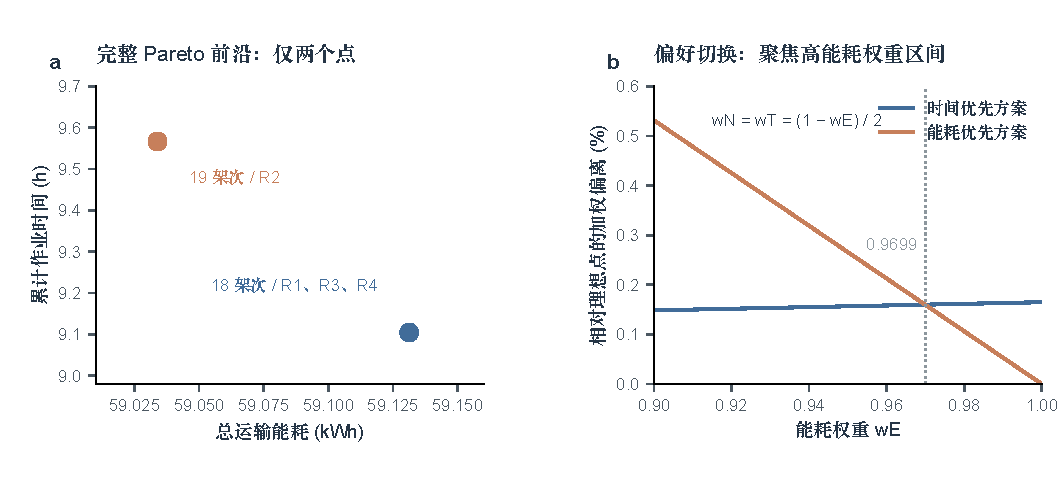
\includegraphics[width=\linewidth]{figures/q1_tradeoff.pdf}
 \caption{完整 Pareto 前沿及偏好切换。左图以真实能耗和累计时间标出两个离散前沿点，架次数直接标注，不连接为可连续插值的方案。右图固定 $w_N=w_T=(1-w_E)/2$，展示高能耗权重区间内的理想点归一化加权偏离；两条曲线相交处为方案切换点。}
 \label{fig:q1-tradeoff}
\end{figure}

\subsubsection{权衡来自何处：S008 的局部替换}

从 $P_T$ 切换到 $P_E$，全局只改变 S008 的组批：将一架 C 型运送全部 $45\,\mathrm{kg}$，替换为两架 B 型分别运送 $25\,\mathrm{kg}$ 和 $20\,\mathrm{kg}$，其他服务区方案保持一致。图~\ref{fig:q1-local}将这项替换展开到货箱层面。B 型分批降低该区能耗，却重复了往返飞行与固定准备、交接过程，因此全局增加 1 架次和 $27.733$ 分钟累计作业时间，仅节省 $0.097354\,\mathrm{kWh}$。

以时间优先方案为基准，能耗节省约 $0.1646\%$，但累计时间增加约 $5.0768\%$、架次数增加约 $5.5556\%$。反过来，选择 $P_T$ 相当于用约 $0.2106\,\mathrm{kWh}$ 的额外能耗换取 1 小时累计作业时间的减少；该比率只是两个离散方案之间的换算，不是连续可调的边际效率，也未给能源与时间设定货币价格。由此，在本问以减少累计作业投入为先的偏好下，推荐 $P_T$；若能源成为压倒性的首要目标，则保留 $P_E$ 作为备选。
\begin{figure}[!htbp]
 \centering
 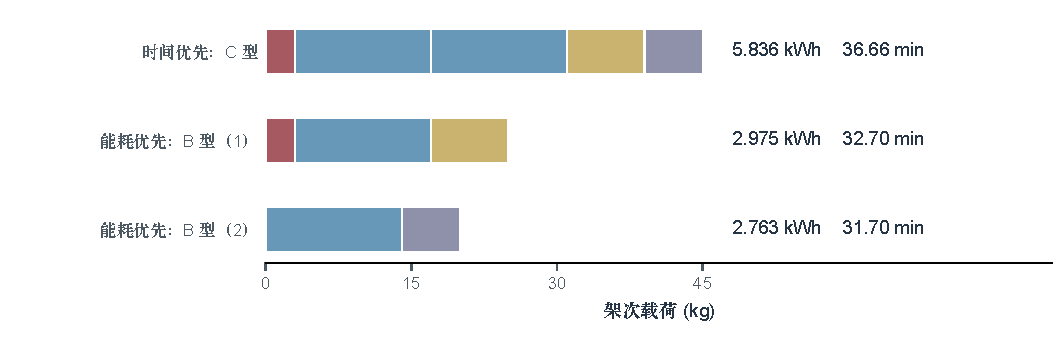
\includegraphics[width=\linewidth]{figures/q1_local_tradeoff.pdf}
 \caption{S008 的局部方案替换解释全局指标冲突。每个色块代表一个不可拆货箱，颜色依次对应医疗物资、饮用水、应急食品、生活卫生用品，与图~\ref{fig:q1-batches}一致；右侧为各架次实际能耗和累计作业时间。}
 \label{fig:q1-local}
\end{figure}

\subsubsection{权重切换边界与推荐的适用范围}

权重分析用于说明推荐对偏好变化的敏感程度，而不是取代字典序决策。将两个前沿点代入式~\eqref{eq:q1-weight}，时间优先点满足 $J(P_T)\le J(P_E)$ 当且仅当
\begin{equation}
 0.00164912\,w_E\le0.05555556\,w_N+0.05076766\,w_T.
 \label{eq:q1-boundary}
\end{equation}
等号上两点并列。该不等式给出整个非负权重单纯形中的选择区域；在 $w_N=w_T$ 的一维截面上，切换点为 $w_E\approx0.969912$。只有当能耗权重高于约 $96.99\%$ 时，该归一化规则才改选 $P_E$。这并不说明能源通常不重要，而是因为本数据下两方案的相对能耗差远小于相对时间和架次差；数值也依赖理想值归一化口径，不能推广为通用阈值。

若决策者愿意接受有限时间增加，也可采用 $\varepsilon$ 约束：先求最小 $T^*$，再在 $T\le T^*+\Delta T$ 下最小化能耗。本数据中，$\Delta T<27.733$ 分钟时只能选择 $P_T$；达到该离散门槛后，$P_E$ 才成为能耗更低的备选。该表述可直接回答“为了节能愿意多投入多少作业时间”，比只列四条规则更明确。

\subsection{推荐组批结果与机型价值}

推荐方案以 B 型 9 架次、C 型 9 架次完成全部 80 箱交付，不使用 A 型。S001、S002、S003 各需两架次，其余服务区各一架次。表~\ref{tab:q1-plan}给出机型、四类货箱数量、质量、体积、能耗和累计作业时间，图~\ref{fig:q1-batches}展示每个不可拆货箱的装载位置。同类型箱号按首批标记与编号顺序映射至批次，但这仅用于生成可核对的箱号清单，不保证后续调度中的首批时限已经满足。
\begin{table}[!htbp]
\centering
\caption{时间优先推荐方案的逐架次装载与代价}
\label{tab:q1-plan}
\small
\setlength{\tabcolsep}{4pt}
\renewcommand{\arraystretch}{1.10}
\begin{tabular}{@{}llcrrrr@{}}
\toprule
架次 & 机型 & 箱数向量 & 质量（kg） & 体积（m$^3$） & 能耗（kWh） & 时间（min） \\
\midrule
S001-1 & C & 2/5/0/0 & 76 & 0.159 & 2.918 & 26.00 \\
S001-2 & C & 0/3/3/2 & 78 & 0.235 & 2.996 & 27.10 \\
S002-1 & B & 1/1/1/0 & 25 & 0.067 & 2.713 & 30.28 \\
S002-2 & C & 0/3/1/1 & 56 & 0.144 & 5.721 & 34.03 \\
S003-1 & B & 1/1/1/0 & 25 & 0.067 & 2.780 & 34.68 \\
S003-2 & C & 0/3/1/1 & 56 & 0.144 & 5.765 & 39.50 \\
S004-1 & C & 1/3/1/1 & 59 & 0.156 & 6.153 & 38.35 \\
S005-1 & C & 1/3/1/1 & 59 & 0.156 & 4.222 & 31.29 \\
S006-1 & C & 1/3/1/1 & 59 & 0.156 & 2.598 & 26.03 \\
S007-1 & C & 1/2/1/1 & 45 & 0.129 & 3.411 & 31.79 \\
S008-1 & C & 1/2/1/1 & 45 & 0.129 & 5.836 & 36.66 \\
S009-1 & B & 1/1/1/0 & 25 & 0.067 & 2.096 & 25.97 \\
S010-1 & B & 1/1/1/0 & 25 & 0.067 & 1.823 & 25.92 \\
S011-1 & B & 1/1/1/0 & 25 & 0.067 & 1.074 & 19.81 \\
S012-1 & B & 1/1/1/0 & 25 & 0.067 & 2.752 & 32.05 \\
S013-1 & B & 1/1/1/0 & 25 & 0.067 & 1.825 & 25.17 \\
S014-1 & B & 1/1/1/0 & 25 & 0.067 & 2.140 & 31.16 \\
S015-1 & B & 1/1/1/0 & 25 & 0.067 & 2.307 & 30.47 \\
\bottomrule
\end{tabular}
\par\smallskip{\footnotesize 箱数向量按医疗物资、饮用水、应急食品、生活卫生用品排列；同一区的架次序号仅用于标识，不表示已完成时序调度。}
\end{table}

\begin{figure}[!htbp]
 \centering
 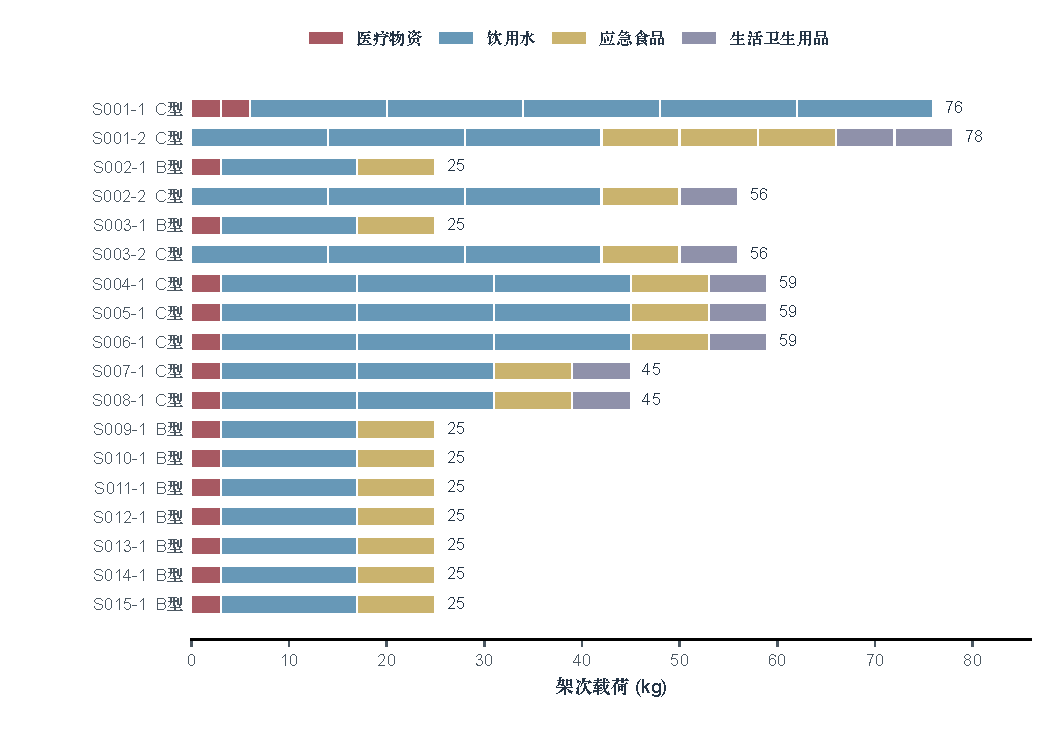
\includegraphics[width=\linewidth]{figures/q1_batches.pdf}
 \caption{时间优先推荐方案的 18 个架次装载组成。每行对应一个架次，每个色块对应一个货箱，色块宽度按单箱质量确定，右侧标注该架次总载荷；行标签包含服务区、架次序号和机型。}
 \label{fig:q1-batches}
\end{figure}

为区分重载能力与混合机型搭配的作用，对仅 A、仅 B、仅 C、A+B 和 A+B+C 五种可用集合均采用同一时间优先规则。表~\ref{tab:q1-policies}及图~\ref{fig:q1-policies}表明，仅 C 已能以 18 架次完成任务，但累计时间为 $9.400\,\mathrm h$、能耗为 $73.935\,\mathrm{kWh}$；允许混合机型后，架次数不变而累计时间降至 $9.104\,\mathrm h$、能耗降至 $59.131\,\mathrm{kWh}$。C 型承担大批量任务，B 型承担较小批量任务，避免在所有航段统一使用大机型。

相较 A+B，增加 C 型可用选项使时间优先方案从 35 架次降为 18 架次，累计时间由 $15.460\,\mathrm h$ 降至 $9.104\,\mathrm h$。这是当前需求、给定机型参数和无实体资源限制条件下的能力对照，并不等于采购收益评价；后续问题二引入实体数量与电池约束后仍需重新调度，不能直接把“B 型 9 架次”解释为需要 9 架 B 型无人机。
\begin{table}[!htbp]
\centering
\caption{统一采用时间优先规则的机型可用集合比较}
\label{tab:q1-policies}
\small
\setlength{\tabcolsep}{4pt}
\renewcommand{\arraystretch}{1.10}
\begin{tabular}{@{}lrrr@{}}
\toprule
机型集合 & 架次数 & 能耗（kWh） & 时间（h） \\
\midrule
A & 52 & 112.180 & 24.813 \\
B & 35 & 68.351 & 15.460 \\
C & 18 & 73.935 & 9.400 \\
A+B & 35 & 68.351 & 15.460 \\
A+B+C & 18 & 59.131 & 9.104 \\
\bottomrule
\end{tabular}
\end{table}

\begin{figure}[!htbp]
 \centering
 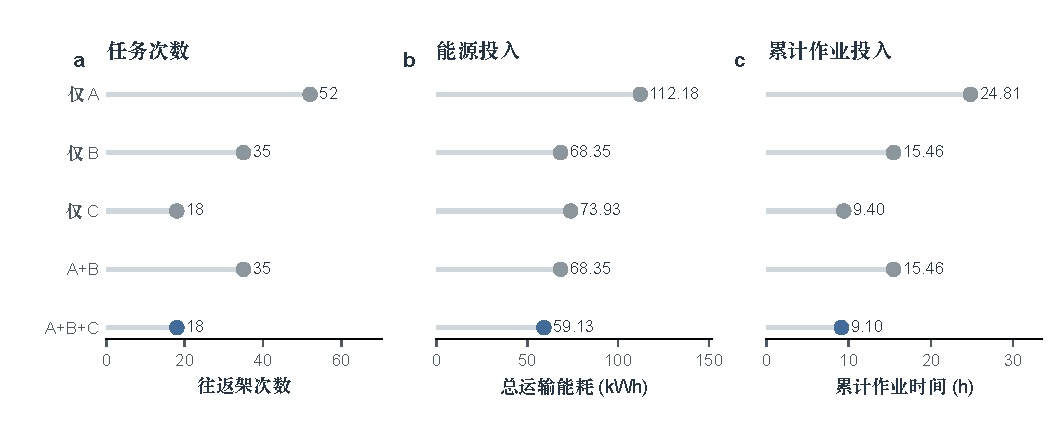
\includegraphics[width=\linewidth]{figures/q1_policies.pdf}
 \caption{五种机型可用集合在相同时间优先规则下的三指标比较。各集合均完整交付 80 箱；蓝色突出 A+B+C 推荐集合。各面板单位不同，不跨面板比较图上长度。}
 \label{fig:q1-policies}
\end{figure}

\subsection{返航安全余量变化的影响}
\subsubsection{连续能力收缩与离散组批跳变}

将三机型返航安全余量统一设为 $\rho$，在 $[0.05,0.45]$ 内以 0.01 步长逐点重新计算最大载荷、可行模式及精确组批，不沿用基准方案。两个机型--服务区临界值分别为
\begin{equation}
 \rho_{gi}^{\rm cap}=1-\frac{E_{gi}(Q_g)}{E_g^{\rm use}},\qquad
 \rho_{gi}^{\rm empty}=1-\frac{E_{gi}(0)}{E_g^{\rm use}}.
 \label{eq:q1-reservelimits}
\end{equation}
前者标志能量约束开始限制满载，后者标志空载往返也无法满足安全余量。在部分载荷区间，$q_{gi}^{\max}$ 随 $\rho$ 连续下降；但货箱不可拆，装载模式只有跨过某个组合质量对应的阈值才会被删除，所以架次数和累计时间呈离散变化。

表~\ref{tab:q1-sensitivity}给出时间优先结果，图~\ref{fig:q1-sensitivity}同时对照能耗优先结果。在固定目标优先规则下，约束收紧使可行域缩小，最小累计时间不可能改善；但时间优先方案的能耗不是单独的最小能耗，其随 $\rho$ 的变化不必单调。该区别解释了图中部分区间的指标不同步，不能仅凭能耗曲线局部下降就认为提高余量改善了整体运输效率。
\begin{table}[!htbp]
\centering
\caption{返航安全余量扫描的时间优先组批结果}
\label{tab:q1-sensitivity}
\small
\setlength{\tabcolsep}{4pt}
\renewcommand{\arraystretch}{1.10}
\begin{tabular}{@{}rrrrl@{}}
\toprule
$\rho$ & 架次数 & 能耗（kWh） & 时间（h） & 完整配送 \\
\midrule
0.05 & 18 & 59.131 & 9.104 & 可行 \\
0.10 & 18 & 59.131 & 9.104 & 可行 \\
0.15 & 18 & 59.131 & 9.104 & 可行 \\
0.20 & 18 & 59.131 & 9.104 & 可行 \\
0.25 & 19 & 61.165 & 9.600 & 可行 \\
0.30 & 20 & 67.228 & 10.163 & 可行 \\
0.35 & 25 & 75.638 & 12.603 & 可行 \\
0.36 & -- & -- & -- & 不可行 \\
0.40 & -- & -- & -- & 不可行 \\
0.45 & -- & -- & -- & 不可行 \\
\bottomrule
\end{tabular}
\par\smallskip{\footnotesize 不可行时不以已覆盖服务区的部分合计冒充全局结果。扫描步长为 0.01，精确边界另由单箱可行性推导。}
\end{table}

\begin{figure}[!htbp]
 \centering
 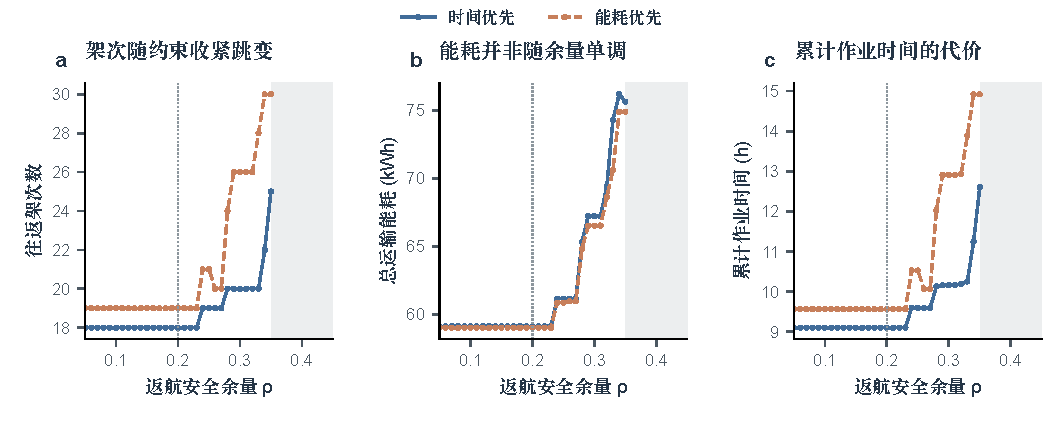
\includegraphics[width=\linewidth]{figures/q1_sensitivity.pdf}
 \caption{返航安全余量对完整配送三指标的影响。各点为间隔 0.01 的重新求解结果，连线仅引导阅读，不代表区间内线性变化；灰区为解析判定的不可完整配送区域，基准余量为 0.20。}
 \label{fig:q1-sensitivity}
\end{figure}

\subsubsection{不可拆单箱决定完整配送的精确边界}

“空载能够往返”是必要但不足的条件。在本问不限制架次数与实体资源的前提下，完整配送可行当且仅当每个货箱都至少能由一种机型单独运输。必要性来自能耗对载荷的单调性：若某箱无法单独运输，加入其他箱也不可能使其可行；充分性来自可以为每箱安排独立架次。因此，令 $\mathcal G_b$ 表示结构载荷与体积均能容纳货箱 $b$ 的机型集合，则统一余量的精确上界为
\begin{equation}
 \rho^*=\min_b\ \max_{g\in\mathcal G_b}
 \left[1-\frac{E_{g,i(b)}(m_b)}{E_g^{\rm use}}\right].
 \label{eq:q1-rhostar}
\end{equation}
若某箱的 $\mathcal G_b$ 为空，则即使不计能量也不可配送；本数据不存在该情形。代入实际附件得到
\begin{equation}
 \rho^*=0.3526780661\approx35.268\%.
 \label{eq:q1-threshold}
\end{equation}
限制来自 S008 的两箱饮用水，每箱 $14\,\mathrm{kg}$；在该临界值处，最有利机型 C 的单箱往返能耗恰好达到预算。基准扫描的 0.35 可行而 0.36 不可行，是这一边界的离散观测，不能把 0.35 当作真正最大值。另在 $\rho^*\pm10^{-6}$ 两侧重新运行组批，结果分别为可行和不可行。

图~\ref{fig:q1-reserve}将 S008 的连续载荷收缩与全部服务区的单箱可行边界联系起来。该上界表示“仍存在完整配送方案”，并不表示接近上界时的架次数与作业时间仍可接受，更不构成应当提高安全余量至上界的运营建议。
\begin{figure}[!htbp]
 \centering
 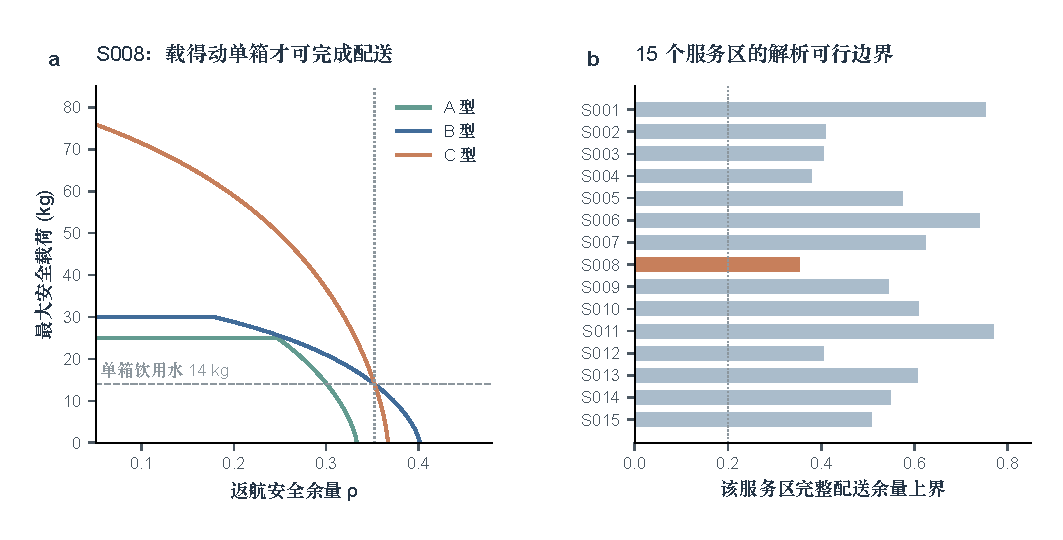
\includegraphics[width=\linewidth]{figures/q1_reserve.pdf}
 \caption{S008 的载荷瓶颈与各服务区完整配送的解析边界。左图虚线表示单箱饮用水质量与全局临界余量；空载不可行后的机型曲线停止。右图以各区最难运输货箱的最佳机型能力确定上界，S008 构成全局瓶颈。}
 \label{fig:q1-reserve}
\end{figure}

\subsection{结果核验与适用边界}

结果检查从几何、连续载荷、组合最优性与逐箱执行四个层面展开。首先，通过直线与像元边界的参数交点法独立重建 15 条航段经过的像元集合，最高高程与原遍历结果一致；其次，45 个基准最大载荷均经独立求根复核。对多目标动态规划的 629 个非零已访问状态，采用直接两两支配判定复查，与前缀最小值筛选所得前沿一致。另从未经模式支配剪枝的原始装载模式建立整数规划，分别核验 15 个服务区的架次数、能耗与时间最优值，共 45 项均与动态规划相符；并在各局部前沿点的架次和时间上界内重新最小化能耗，得到相同结果。

对四种决策规则生成的实际箱号方案，逐架次从原始货箱重新汇总质量与体积，独立代入能耗和时间公式，确认每箱恰好交付一次、不跨服务区且满足质量、体积和返航余量要求。这些检查支持给定离散模型内的结果，不能消除 DEM 分辨率、附件参数以及统一能耗公式本身的适用限制。全部求解为确定性过程，不把随机重复次数或人为误差条当作验证证据。

本问的主要结论是：采用时间优先规则可得到 18 架次完整配送方案，其与能耗最优方案的差异可归因于 S008 的局部机型替换；较小的节能幅度伴随明确的额外作业代价。安全余量的影响则分为连续载荷下降、离散合批变化和单箱不可行三个层次。后续调度应继承公共几何与物理计算口径，但在引入多点航线、实体资源和时限后重新求解，不能把本问累计时间或组批最优性直接移作调度结论。
